%%
%% This is file `sample-sigconf.tex',
%% generated with the docstrip utility.
%%
%% The original source files were:
%%
%% samples.dtx  (with options: `sigconf')
%% 
%% IMPORTANT NOTICE:
%% 
%% For the copyright see the source file.
%% 
%% Any modified versions of this file must be renamed
%% with new filenames distinct from sample-sigconf.tex.
%% 
%% For distribution of the original source see the terms
%% for copying and modification in the file samples.dtx.
%% 
%% This generated file may be distributed as long as the
%% original source files, as listed above, are part of the
%% same distribution. (The sources need not necessarily be
%% in the same archive or directory.)
%%
%% The first command in your LaTeX source must be the \documentclass command.
% \documentclass[sigconf]{acmart}
\documentclass[sigconf,review,nonacm]{acmart}
% \usepackage{algorithm}
% \usepackage{algorithmicx}
\usepackage[ruled]{algorithm2e}
\usepackage{algpseudocode}
\usepackage{amsmath}
\usepackage{subfigure}
\usepackage{enumitem}
\usepackage{multirow}
\usepackage{pifont}
%% NOTE that a single column version may be required for 
%% submission and peer review. This can be done by changing
%% the \doucmentclass[...]{acmart} in this template to 
%% \documentclass[manuscript,screen]{acmart}
%% 
%% To ensure 100% compatibility, please check the white list of
%% approved LaTeX packages to be used with the Master Article Template at
%% https://www.acm.org/publications/taps/whitelist-of-latex-packages 
%% before creating your document. The white list page provides 
%% information on how to submit additional LaTeX packages for 
%% review and adoption.
%% Fonts used in the template cannot be substituted; margin 
%% adjustments are not allowed.
%%
%%
%% \BibTeX command to typeset BibTeX logo in the docs
\AtBeginDocument{%
  \providecommand\BibTeX{{%
    \normalfont B\kern-0.5em{\scshape i\kern-0.25em b}\kern-0.8em\TeX}}}

%% Rights management information.  This information is sent to you
%% when you complete the rights form.  These commands have SAMPLE
%% values in them; it is your responsibility as an author to replace
%% the commands and values with those provided to you when you
%% complete the rights form.
\setcopyright{acmcopyright}
\copyrightyear{2021}
\acmYear{2021}
\acmDOI{10.1145/1122445.1122456}
\settopmatter{printacmref=false} % Removes citation information below abstract
\renewcommand\footnotetextcopyrightpermission[1]{} % removes footnote with conference information in first column
\pagestyle{plain} % removes running headers

%%
%% Submission ID.
%% Use this when submitting an article to a sponsored event. You'll
%% receive a unique submission ID from the organizers
%% of the event, and this ID should be used as the parameter to this command.
%%\acmSubmissionID{123-A56-BU3}

%%
%% The majority of ACM publications use numbered citations and
%% references.  The command \citestyle{authoryear} switches to the
%% "author year" style.
%%
%% If you are preparing content for an event
%% sponsored by ACM SIGGRAPH, you must use the "author year" style of
%% citations and references.
%% Uncommenting
%% the next command will enable that style.
%%\citestyle{acmauthoryear}


\begin{document}


\title{Adaptive Hyperbolic Graph Neural Network via Multi-Agent Reinforcement Learning}
% \renewcommand{\title}{Adaptive Hyperbolic Graph Neural Network via Reinforcement Learning}



%%
%% By default, the full list of authors will be used in the page
%% headers. Often, this list is too long, and will overlap
%% other information printed in the page headers. This command allows
%% the author to define a more concise list
%% of authors' names for this purpose.
\renewcommand{\shortauthors}{}


\begin{abstract}
Graph Neural Networks (GNNs) have been widely studied in various graph data mining tasks. 
Most existing GNNs embed graph nodes in Euclidean space and thus are less effective to capture the ubiquitous hierarchical structure in real-world networks. 
Hyperbolic Graph Neural Networks (HGNNs) extend GNNs to hyperbolic space and obtains more powerful node representation capability of the graph with hierarchical structures. 
In hyperbolic geometry, the graph hierarchical structure can be reflected by the curvatures of the hyperbolic space, and different curvatures can model different hierarchical structures of a graph. 
However, most existing HGNNs set the curvature to a fixed value for simplicity, which may not perform well for graphs with complex and diverse hierarchical structure. 
To solve this problem, we for the first time study the adaptive hyperbocil graph neural network model to adaptively learn the optimal curvature according to the input graph. 
We propose RAHGNN, a multi-agent reinforcement learning based framework for building the adaptive hyperbolic graph neural network. Specifically, RAHGNN contains two agents, ACE-Agent and HGNN-Agent for learning the curvature and node representations, respectively. The two agents are updated by a Nash Q-leaning algorithm collaboratively, seeking for the better hyperbolic space indexed by the curvature. 
Extensive experiments on multiple real-world graph datasets demonstrate a significant and consistent improvement in model quality with competitive performance and good generalization ability. 
\end{abstract}


%%
%% The code below is generated by the tool at http://dl.acm.org/ccs.cfm.
%% Please copy and paste the code instead of the example below.
%%
% \begin{CCSXML}
% <ccs2012>
%  <concept>
%   <concept_id>10010520.10010553.10010562</concept_id>
%   <concept_desc>Computer systems organization~Embedded systems</concept_desc>
%   <concept_significance>500</concept_significance>
%  </concept>
%  <concept>
%   <concept_id>10010520.10010575.10010755</concept_id>
%   <concept_desc>Computer systems organization~Redundancy</concept_desc>
%   <concept_significance>300</concept_significance>
%  </concept>
%  <concept>
%   <concept_id>10010520.10010553.10010554</concept_id>
%   <concept_desc>Computer systems organization~Robotics</concept_desc>
%   <concept_significance>100</concept_significance>
%  </concept>
%  <concept>
%   <concept_id>10003033.10003083.10003095</concept_id>
%   <concept_desc>Networks~Network reliability</concept_desc>
%   <concept_significance>100</concept_significance>
%  </concept>
% </ccs2012>
% \end{CCSXML}

% \ccsdesc[500]{Computer systems organization~Embedded systems}
% \ccsdesc[300]{Computer systems organization~Redundancy}
% \ccsdesc{Computer systems organization~Robotics}
% \ccsdesc[100]{Networks~Network reliability}

%%
%% Keywords. The author(s) should pick words that accurately describe
%% the work being presented. Separate the keywords with commas.
\keywords{Hyperbolic Geometry, Graph Neural Network, Reinforcement Learning, Complex Network}


%%
%% This command processes the author and affiliation and title
%% information and builds the first part of the formatted document.
\maketitle



\section{Introduction}
%Background%
Graphs have been widely used to model the complex relationships between objects, such as social networks~\cite{hamilton2017inductive}, academic networks~\cite{getoor2005link}, and biological networks~\cite{gilmer2017neural}. 
In recent years, graph representation learning has shown its effectiveness in capturing the irregular but related complex structures in graph data~\cite{hamilton2017inductive}. 
As an important topology characteristic, hierarchical structures are ubiquitous in many real-world graphs, such as the hypernym structure in natural languages~\cite{NickelK17Poincare,PoincareGlove}, the subordinate structure of entities in the knowledge graph~\cite{balazevic2019multi,wang2020h2kgat}, and the cascade structure of information propagation in social networks~\cite{zubiaga2018detection}. 
In our work, we focus on studying the tree-like structure\footnote{We interchangeably use the terms \textit{heirarchy} and \textit{tree-like structure} in this paper. } which exists extensively in real-world networks~\cite{Krioukov2010Hyperbolic}. 


\begin{figure}[ht]
	\centering
	\includegraphics[width=0.45\textwidth]{figure/example_1.png}
	\caption{An example of a hyperbolic distance (\textcolor{red}{dash line}) between two nodes on a binary tree in hyperbolic spaces with different curvatures}
	\label{example_1}
\end{figure}

%Weaknesses of exiting works%
With the advantages of better capturing the hierarchical structures of graphs compared with the Euclidean space, hyperbolic space has been introduced into Graph Neural Networks to achieve better learning performance and interpretability~\cite{NickelK17Poincare}. 
To learn the graph representations in hyperbolic space, Hyperbolic Graph Neural Networks (HGNNs) extend the node feature aggregation of Graph Neural Networks (GNNs) into hyperbolic space. 
HGNNs combine hyperbolic geometric embedding and GNNs, and effectively fuse the node features and the hierarchical structures to acquire the superior node representation for graphs. 

However, a major limitation of existing HGNNs is that they cannot adaptively choose the appropriate hyperbolic space to represent the graphs with different degrees of tree-like structures.
Thus, even though most real-world graphs have tree-like structures, they have different degrees of ``how tree-like a graph is''. 
In this paper, we use Gromov’s $\delta$-hyperbolicity~\cite{adcock2013tree} to measure the degree of tree-like structures of a graph. 
Existing HGNNs provide great expressiveness for high hyperbolicity (more like a tree) graph data, but it shows poor performance in node representation of graphs with low hyperbolicity (less like a tree) ~\cite{HGCN_ChamiYRL19}. 


%Problem presentation%
To investigate this problem, we review hyperbolic geometry and related studies~\cite{cannon1997hyperbolic,Krioukov2010Hyperbolic}, and we were inspired by the curvature which can be used to measure any hyperbolic geometry similarity to Euclidean geometry.
We illustrate an intrinsic connection between hyperbolic curvature and hierarchies of graphs in Figure~\ref{example_1}. 
The examples show that different curvatures significantly affect distance metric in hyperbolic space. 
We can observe that the hyperbolic distance between two nodes in different hyperbolic spaces is approximately equal to the length of shortest path in the tree or the Euclidean distance.
In deep learning frameworks, HNN~\cite{HNN:GaneaBH18} presents that with the curvature going to zero, the hyperbolic distance metric is approximate identical to the Euclidean distance metric. 
The distance measures determine the retention of the hierarchy when embedding graphs into hyperbolic spaces with different curvatures. 
Therefore, a natural problem is, “\textit{Can we make a hyperbolic geometric learning model automatically learn the appropriate curvature to obtain desirable adaptability for different graphs with tree-like structure?}” 

%Challenges%
However, there are two major challenges to adaptively find the optimal hyperbolic curvature to improve the learning ability of HGNNs. 
The one is learning curvature and node representation together may lead to training instability since the updating curvature will continuously change the entire hyperbolic embedding space. 
Existing work~\cite{HGCN_ChamiYRL19} takes curvature as a parameter to learn node representations of the graph. However, instead of learning the accurate curvature in training process, it only slightly adjusts the curvature to make the node representation learning converge in a relatively stable hyperbolic space.
The other one is learning curvature with optimization methods is difficult because there is no strict and formal mathematical method to map curvature and hierarchy of the graph, which can change the hierarchy-preserving capability of hyperbolic space through different distance metric. 



%Proposed method%
To address the above challenges, we propose a novel \textbf{A}daptive \textbf{H}yperbolic \textbf{G}raph \textbf{N}eural \textbf{N}etwork via Multi-Agent \textbf{R}einforcement Learning named \textbf{RAHGNN}. 
The basic idea is that we take the downstream task as the environment in reinforcement learning and calculate the feedback reward based on the hyperbolic node representations.
Specifically, we design two agents: the adaptive curvature explore agent (ACE-Agent) and the hyperbolic graph neural network agent (HGNN-Agent). 
The adaptive curvature explore agent (ACE-Agent) is designed to independently learn the optimal curvature in a broad range of the parameter space based on reinforcement learning. 
The hyperbolic graph neural network agent (HGNN-Agent) with variable curvature is designed to learn the node representations in hyperbolic space with a particular curvature. 
To fully ensure learning both curvature exploration and graph representations in hyperbolic space, we propose a multi-agent reinforcement learning framework to learn curvature and node representations collaboratively. 
The optimized goal is the two cooperative agents have a Nash equilibrium. 
In this way, the curvature can adaptively adjust to the distance metric of embedded space for different graphs with complex hierarchical topologies.
Extensive experiments on typical real-world datasets demonstrate a significant and consistent improvement in model quality with competitive performance. 
We have also visualized the graph in hyperbolic space to provide an intuitive understanding of how different curvatures affect the model's capability of capturing the hierarchy. 
We summarize our contributions as follows: 
\vspace{-0.4em}
\begin{itemize}[leftmargin=*]
\item We make a observation and analysis of the adaptability problem of GNNs to graphs with different hierarchical topologies in hyperbolic space, and we transform the adaptability problem into an optimal curvature exploration problem in hyperbolic space. 
\item We propose a novel hyperbolic graph representation learning framework with superior adaptive capability based on multi-agent reinforcement learning. 
To our best knowledge, it is the first attempt to utilize reinforcement learning in hyperbolic machine learning. 
\item To solve the two key problems of learning curvature and HGNN at the same time, we design the ACE-Agent and HGNN-Agent to learn the curvature and HGNN respectively, and cooperatively train their rewards to reach Nash equilibrium based on multi-agent reinforcement learning. 

\end{itemize}


\section{Hyperbolic Geometric Models}
Hyperbolic space commonly refers to manifolds with constant negative curvature and is used for modeling complex networks.
In hyperbolic geometry, there are five common isometric models used to describe hyperbolic spaces~\cite{cannon1997hyperbolic}. 
Among them, the Poincaré model, Hyperboloid (Lorenz) model, and Klein model have recently been used in machine learning for preserving different kinds of hierarchies in graphs~\cite{NickelK17Poincare,PoincareGlove,HNN:GaneaBH18,HGNN_Qi,HAtt}. 

\subsection{Poincaré Ball Model}
The Poincaré ball model is a $n$-dimensional model of hyperbolic geometry with nodes located in the unit ball interior, and the 2-dimensional is the Poincaré disk. 
The distance on this manifold with standard negative constant curvature $K=-1$ is defined as: 
\begin{equation}\label{equ:1}
\begin{aligned}
d_{p}(\mathbf{x}, \mathbf{y})=\operatorname{arccosh}\left(1+2 \frac{\|\mathbf{x}-\mathbf{y}\|^{2}}{\left(1-\|\mathbf{x}\|^{2}\right)\left(1-\|\mathbf{y}\|^{2}\right)}\right), 
\end{aligned}
\end{equation}
where $\mathbf{x}$, $\mathbf{y}$ are the nodes inside the Poincaré Ball. 

\subsection{Hyperboloid Model}
The hyperboloid (Lorentz) model is a model of $n$-dimensional hyperbolic geometry as a manifold in the $(n+1)$-dimensional Minkowski space. 
The hyperboloid model consists of $\mathcal{H}^n= \{ x\in \mathcal{R}^{n+1} \mid  \langle x,x \rangle_{\mathcal{M}} = K, x_{0}>0 \}$, where $\langle x,x \rangle_\mathcal{L}$ is the Lorentzian scalar product, $K$ is the curvature, and the distance $d_{\mathcal{H}}(x,y)$ on the hyperboloid model between two points $x$ and $y$ in hyperbolic space with standard hyperbolic curvature $K=-1$ is: 
\begin{equation}
\label{equ:2}
\begin{aligned}
     d_{\mathcal{H}}(\mathbf{x},\mathbf{y})= \langle \mathbf{x},\mathbf{y} \rangle_{\mathcal{L}} = \mathrm{arccosh}({x_0 y_0} - \sum_{i=1}^{n}{x_i y_i}), 
\end{aligned}
\end{equation}
where  $\mathbf{x}$, $\mathbf{y}$ are the nodes inside the $(n+1)$-dimensional Minkowski space. 

\subsection{Klein Model}
Klein model is a projective model of hyperbolic geometry in which points are represented by the points in the interior of the unit disk (or ball), and lines are represented by the chords. 
The Klein model is defined on $\mathcal{K}^n$ $= \{\mathbf{x} \in \mathcal{R}^n \mid \|\mathbf{x}\| < 1 \}$ , and it can be transformed between the hyperboloid model and the Klein model: 
\begin{equation}\label{equ:3}
\begin{aligned}
    &\pi_{\mathcal{H} \to \mathcal{K}}(\mathbf{x})=\frac{(x_0,...,x_i)}{x_{0}}, \\
    &\pi_{\mathcal{K} \to \mathcal{H}}(\mathbf{x})=\frac{1}{\sqrt{1-\| \mathbf{x} \|^2}}.
\end{aligned}
\end{equation}

\begin{figure*}[t]
\centering
\subfigure[]{
\includegraphics[width=0.24\linewidth]{figure/fig1_a.png}
\label{example:a}
%\caption{fig1}
}%
\subfigure[]{
\includegraphics[width=0.24\linewidth]{figure/fig1_b.png}
\label{example:b}
%\caption{fig2}
}%
\subfigure[]{
\includegraphics[width=0.52\linewidth]{figure/fig1_c.png}
\label{example:c}
}
\centering
\caption{An illustration of different distance metrics in hyperbolic spaces with different curvature. 
(a) Graph distance (\textcolor{purple}{purple solid lines}), Euclidean distance (\textcolor{blue}{blue dashed}) and hyperbolic geodesics(\textcolor{red}{red dashed curve}) on a tree-like graph in Poincaré disk; 
(b) Graph distance and embedded distance in Poincaré disk (Euclidean projection, \textcolor{blue}{blue solid and dashed lines}) and hyperboloid (Curvature $K = -1$ \textcolor{red}{red solid and dashed curves}); 
(c) Graph distance and hyperbolic distance on the hyperboloid of different curvature. }
\label{example}
\end{figure*}

\section{Curvature versus Hierarchical Structure}
\label{section 3}
In this section, we perform a qualitative analysis to reveal the intrinsic connections between curvature and the hierarchical structure. 
We illustrate a hyperbolic space tree-like graph as an example on Poincaré disk as shown in Figure~\ref{example:a}. 
To help explain our observation, we define two important distances as follows: 

%Distance introduction%
\textbf{Graph distance. }
Graph distance represents the length of the shortest path between two nodes on a graph.
Propagating information is an essential function of many real networks (e.g., Internet, brain, regulatory, metabolic networks). 
We can use information propagation to measure the topological distance between two nodes in graph representation learning. 
The graph distance $\mathbf{g_{i j}}$ between node $i$ and node $j$ is defined as follows: 
\begin{equation}\label{graphdist}
    \mathbf{g}_{i j} = \mathbf{d}_{i k_1} + \mathbf{d}_{k_1 k_2} + \mathbf{d}_{k_2 k_3} + \cdots + \mathbf{d}_{k_n j},
\end{equation}
where $k_1,k_2,\cdots,k_n$ are the nodes on the shortest path between node $i$ and node $j$, and $\mathbf{d}$ is the embedded distance between two nodes. 
In the Figure~\ref{example:a}, the graph distance between nodes $A$ and $D$ (\textcolor{purple}{purple solid lines}) is $\mathbf{g}_{AD}=r_{AB}+r_{BC}+r_{CD}$. 

\textbf{Embedded distance. }
Embedded distance represents the distance between two nodes in the embedded space (dashed lines in Figure~\ref{example}), which can be regarded as the semantic distance or feature similarity between two nodes in machine learning. 
We use $\mathbf{d}_{\mathcal{E}}$ and $\mathbf{d}_{\mathcal{H}}$ to denote the embedding distance in Euclidean and hyperbolic embedding spaces, which can be computed by the inner product and the Lorentzian scalar product, respectively. 
The example is shown in Figure~\ref{example:a}. 
For the nodes $A$ and $D$, their Euclidean embedded distance is $\mathbf{d}_{^{AD}\mathcal{E}}$ (\textcolor{blue}{blue dash line}), and the hyperbolic distance is $\mathbf{d}_{^{AD}\mathcal{H}}$ (\textcolor{red}{red dash curve}). 

%Distance computation%
Now, we show how hyperbolic distance changes with curvature as follows. 
Here, we employ the following conclusions from the existing work of hyperbolic geometry in complex network~\cite{Krioukov2010Hyperbolic} to analyze the hyperbolic distance metrics: 
The hyperbolic space of constant curvature is defined as $K = -{\zeta}^2 < 0, \zeta > 0$. 
The hyperbolic distance $\mathbf{d}_{\mathcal{H}}$ between two nodes at polar coordinates $(r, \theta)$ and $(r^{\prime}, \theta^{\prime})$ is given by the hyperbolic law of cosines:
\begin{equation}\label{hyperdist1}
   \cosh \zeta \mathbf{d}_{\mathcal{H}}=\cosh \zeta r \cosh \zeta r^{\prime}-\sinh \zeta r \sinh \zeta r^{\prime} \cos \Delta \theta,
\end{equation}
where $\Delta\theta$ is the angle between the nodes, and this equation converge to their familiar Euclidean analogs, that is $\mathbf{d}_{\mathcal{H}} \rightarrow \mathbf{d}_{\mathcal{E}}$ at $\zeta \rightarrow 0$. 
For sufficiently large $\zeta~r, \zeta~r^{\prime}$, and $\Delta\theta > 2\sqrt{e^{-2~\zeta~r}-e^{-2~\zeta~r'}}$, the hyperbolic distance $x$ can be closely approximated by: 
\begin{equation}\label{hyperdist2}
   \mathbf{d}_{\mathcal{H}}=r+r^{\prime}+\frac{2}{\zeta} \ln \sin \frac{\Delta \theta}{2} \approx r+r^{\prime}+\frac{2}{\zeta} \ln \frac{\Delta \theta}{2}.
\end{equation}
The hyperbolic distance $\mathbf{d}_{\mathcal{H}}$ between two nodes is approximately the sum of their radius and minusing some $\Delta\theta$-dependent correction, and $\Delta\theta \rightarrow 0$ at $\zeta \rightarrow \infty$. 

According to the hyperbolic distance properties above, we can quantitatively analyze the intrinsic connections between the curvature and the distance metrics. 
We denote $(r_1, \theta_1),(r_2, \theta_2),\cdots,(r_n, \theta_n)$ as a node set on the shortest path between $(r, \theta)$ and $(r^{\prime}, \theta^{\prime})$. 
According to Equation~\eqref{graphdist} and Equation~\eqref{hyperdist2}, we can derive the hyperbolic graph distance $\mathbf{g}_{\mathcal{H}}$ as follows:
\begin{equation}\label{hypergraphdist}
   \mathbf{g}_{\mathcal{H}}= r + r^{\prime} + 2\sum_{m=1}^{n}r_m + \frac{2(n+1)}{\zeta}\sum_{k=1}^{n+1}\ln \frac{\Delta \theta_k}{2},
\end{equation}
where $\Delta \theta_k$ is the angle of each node pair on the shortest path. 
With the curvature parameter $\zeta \rightarrow \infty$ and $\Delta \theta_k \rightarrow 0$, we can obtain:
\begin{equation}\label{hypergraphdist2}
   \mathbf{g}_{\mathcal{H}}= \mathbf{d}_{\mathcal{H}} + 2\sum_{m=1}^{n}r_m.
\end{equation}

%Derivation and analysis%
As we all know, a key property of hyperbolic spaces is that hyperbolic spaces expand exponentially while Euclidean spaces expand polynomially~\cite{Krioukov2010Hyperbolic}.
In a tree-like graph, the shortest path navigation between two nodes tends to be close to the center. 
If the graph is more tree-like, the second term is smaller in Equation~\eqref{hypergraphdist2}, and the graph distance $\mathbf{g}_{\mathcal{H}}$ is more closely approximated to the embedded distance $\mathbf{d}_{\mathcal{H}}$.
An example of this visualization is shown in Figure~\ref{example:c}.
with the $|K|$ increases, we can observe two results in the illustration: 
(1) The embedded distance $\mathbf{d}_{^{AD}\mathcal{H}}$ gradually approximates to the graph distance $\mathbf{g}_{^{AD}\mathcal{H}}$ between nodes $A$ and $D$ in the hyperbolic space.
(2) Both $\mathbf{d}_{^{AD}\mathcal{H}}$ and $\mathbf{g}_{^{AD}\mathcal{H}}$ approach the center of hyperboloid. 

%Explaining reasons%
In addition, the illustration showed another essential property of hyperbolic geometry, which can explain why non-tree-like structures cannot be preserved in hyperbolic spaces. 
The sum of the interior angles of a triangle in a space of negative constant curvature is less than $\pi$. 
As shown in Figure \ref{example:c}, the sum of the interior angles decreases with the $|K|$ increases. 
This property can be easily generalized to any cycle structures such as rectangles or trapezoids. 
The real-world graphs often include various cycle structures, such as a triangle describing a simple family relationship, or a ring road of the traffic network. 
For the low hyperbolicity graph with many cycle structures, we adjust a lower curvature value $|K|$ to reduce this structural information loss in hyperbolic space. 

\begin{figure*}[htb]
\centering
\includegraphics[width=0.9\textwidth]{figure/overall.png}
\caption{An illustration of RAHGNN architecture.}
\label{framework}
\end{figure*}

%Summary%
In summary, 
% with the curvature parameter $\zeta = \sqrt{ -K }$ and Equations~\eqref{graphdist},~\eqref{hyperdist2},  and~\eqref{hypergraphdist2}, 
we highlight two important conclusions as follows:
(1) Curvature determines the distance measure by adjusting for the distortion of space, which can measure representations capability with fusing the hierarchical structure and node features information in hyperbolic embedding space. 
(2) For hyperbolic geometric embedding, adjusting the curvature can better capture the hierarchy of the graph. 
However, an inappropriate curvature may degrade the representational capability of node features or semantics, especially in some classification tasks where node features are more important or using some "low tree-like" graphs. 

Based on these properties of curvature, we can solve the structural adaptive problem of hyperbolic graph representation learning as an optimal curvature selection problem of hyperbolic space. 
It provides a foundation for us to design an intuitive and effective solution. 

\section{Reinforcement Learning Based Adaptive Hyperbolic Graph Neural Network}\label{section 4}

In this section, we introduce the proposed RAHGNN, an Adaptive Hyperbolic Graph Neural Network, for node hyperbolic representation learning. 
The overall architecture of RAHGNN is shown in Figure~\ref{framework}. 
We design the HGNN module to learn the node representation in hyperbolic space with a given curvature, and design the adaptive curvature exploration module to explore the curvature of hyperbolic space which can get the maximum reward reward from downstream task.
Then, we present a collaborative reinforcement learning framework with two agents  Hyperbolic Graph Neural Network Agent (HGNN-Agent) and the Adaptive Curvature Exploration agent (ACE-Agent) satisfying Nash equilibrium. 

\subsection{Hyperbolic Graph Neural Network Agent}
The goal of Hyperbolic Graph Neural Network Agent (HGNN-Agent) is to learn the fusing representation of graph structure and node features with a given curvature. 
It focuses on how to integrate the structure information and node features of a graph. 

\subsubsection{HGNN with Variable Curvature}
Though many hyperbolic embedding methods using hyperboloid (Lorentz) models have proved their success in feature representation, they are mostly based on the assumption that the hyperboloid has a constant curvature. 
Therefore, to achieve our goal, we need to extend the hyperbolic graph neural network into a variable curvature version.
A hyperbolic graph neural network layer with variable curvature consists of the three operations as follows:

\paragraph{Hyperbolic Activation with Variable Curvature}
For graph node Euclidean embeddings $x = (x_1, x_2, \dots, x_n) \in \mathcal{R}^{n} $, we first transform the $n$-dimensional vector to the $(n+1)$-dimensional space in pseudo-polar coordinate as follows:
\begin{equation}\label{equ:7}
    x \rightarrow x_{\mathcal{L}}^{K} = (\zeta \left\|x\right\|,\frac{x}{\zeta \left\|x\right\|}).
\end{equation}
Then, the exponential map $\mathrm{exp}^{K}_{x}:\mathcal{E}^n \rightarrow \mathcal{L}^{n+1}$ with curvature $K$ can be defined as: 
\begin{equation}\label{equ:11}
    \mathrm{exp}^{K}_{\mathcal{L}}: \mathbf{h}^{\zeta}_{x \mathcal{L}}=(\cosh{\zeta \left\|\mathbf{h}_x\right\|}, \sinh{\zeta \left\|\mathbf{h}_x\right\|} \frac{\mathbf{h}_x}{\zeta \left\|\mathbf{h}_x\right\|}), 
\end{equation}
where $\mathbf{h}^{\zeta}_{j \mathcal{L}}$ is the projection on hyperboloid of a node hidden state $h_v$. 

For the hyperboloid (Lorentz) model, we consider the Lorentzian scalar product of a Riemannian manifold with curvature $K$ is:
\begin{equation}\label{equ:6}
    \langle x,x \rangle_\mathcal{L} : K x_0^2 + \sum_{i=1}^{n}{x_i^2} = K, 
\end{equation}
where $x_0 = \sqrt{1-\frac{x^2}{K}}$. 
To make the calculation easier, we linearly approximate $x$ in Equation~\eqref{equ:6} to $x = \|x\|/\zeta$, where the $\zeta$ is the curvature parameter, given by $K = -\zeta^2 < 0, \zeta > 0$.

Since we have given the variable curvature version of hyperbolic distance between node $i$ and node $j$ with curvature $K$, and the distance between the node-pair $(i, j)$ on hyperboloid by Equation~\eqref{equ:2}:
\begin{equation}\label{equ:Hdist}
    \mathbf{d}^{K}_{\mathcal{L}}(i,j) = \mathrm{arccosh}{(- \langle \mathbf{h}^{\zeta}_{i \mathcal{L}},\mathbf{h}^{\zeta}_{j \mathcal{L}})\rangle}_{\mathcal{L}}).
\end{equation}

\paragraph{Hyperbolic Attention Aggregation with Variable Curvature}
We next discuss how to conduct the adaptive hyperbolic attention mechanism to aggregate node features by appropriate curvature. 

The GNNs models usually use convolution layers or attention layers to aggregate node feature information. 
As discussed in the previous Section~\ref{section 3}, our goal is to obtain an aggregation with variable curvature in hyperbolic space. 
Therefore, we extend the hyperbolic attention network~\cite{HAtt}, and present a hyperbolic attention aggregation with variable curvature through the following steps.

\textbf{Step-1: }
Considering the variable curvature, given the feature vectors $\mathbf{h}_i$ and $\mathbf{h}_j$ of nodes $i$ and $j$ in Euclidean space, we perform self-attention on the nodes, and the hyperbolic attention weight $\alpha\left(\mathbf{h}_{i}, \mathbf{h}_{j}, K \right)$ can be calculated as follows:
\begin{equation}
    \alpha\left(\mathbf{h}_{i}, \mathbf{h}_{j}, K \right)=\mathrm{exp}\left(-\beta \mathbf{d}^{K}_{\mathcal{L}}(i,j)-b\right),
\end{equation}
where $\pi(\mathbf{h}_{i})$ is the hyperbolic embedding given by Equation~\eqref{equ:7}, and $\mathbf{d}^{\zeta}_{\mathrm{H}}(\cdot,\cdot)$ is the variable curvature hyperbolic distance given by Equation~\eqref{equ:Hdist}. 
Then, we transform these node embeddings $\mathrm{exp}^{K}_{\mathcal{L}}(\mathbf{h})$ to the Klein model, which can represent the node embedding in the interior of the unit disk by Equation~\eqref{equ:11}. 
The hyperbolic embedding of node $v$  in Klein model is defined as:
\begin{equation}
    \mathbf{h}^{\zeta}_{x \mathcal{L}} \rightarrow \mathbf{h}_{x \mathcal{K}}^{\zeta} = \frac{\sinh(\zeta \left\|\mathbf{h}_x\right\|) \mathbf{h}_x}{\zeta \left\|\mathbf{h}_x\right\| \cosh(\zeta \left\|\mathbf{h}_x\right\|)}. 
\end{equation}

\textbf{Step-2:} Then we can utilize the Einstein midpoint in hyperbolic space to compute the weight sum operation in Euclidean space: 
\begin{equation}
    \mathbf{h}_{i \mathcal{K}}^{\zeta} = \sum_{j}\left[\frac{\alpha_{i j} \gamma\left(\mathbf{h}_{j \mathcal{K}}^{\zeta}\right)}{\sum_{\ell} \alpha_{i \ell} \gamma\left(\mathbf{h}_{j \mathcal{K}}^{\zeta}\right)}\right] \mathbf{h}_{j \mathcal{K}}^{\zeta},
\end{equation}
where the Lorentz factors is $\gamma(\mathbf{h}_{j \mathcal{K}}^{\zeta})=\frac{1}{\sqrt{1-  \frac{\sinh^2(\zeta  \left\|\mathbf{h}_j\right\|)}{\cosh^2(\zeta \left\|\mathbf{h}_j\right\|)}    } }$. 

\paragraph{Riemannian Optimization with Variable Curvature}
Since the curvature is a variable parameter, the optimizer needs to be extended accordingly. 
In the hyperboloid model, Riemannian-SGD (RSGD)~\cite{DBLP:conf/icml/NickelK18} is widely used for optimization. 
In the following, we also present a variable curvature version of RSGD with curvature parameter $\zeta$. 
\begin{equation}
\begin{aligned}
    \mathbf{h}^t & = g_{\theta_t}^{-1} \nabla f(\theta), \\ 
    \mathrm{grad}f(\theta_t) & = f(\mathbf{h}^t) + \frac{\langle \mathbf{h}^t,\theta_t \rangle_{\mathcal{L}}}{\zeta^2}\theta_t,  \\ 
    \theta_{t+1} & = \mathrm{exp}_{\theta_t}(-\eta \mathrm{grad}f(\theta_t)).
\end{aligned}
\end{equation}
The initialized embeddings $\mathbf{h}^t$ are close to the origin of $\mathcal{H}^n$ by sampling from the uniform distribution $\mathcal{U}(-0.001, 0.001)$ and by setting $x_0 = \sqrt{1+\frac{x^2}{\zeta^2}}$ according to Equation~\eqref{equ:6}.

\subsubsection{HGNN Agent}
Given a graph $G$ with the adjacency matrix $A$ and the Euclidean feature $X$, the first layer of HGNN maps from Euclidean to hyperbolic space, then the HGNN stacks multiple hyperbolic graph attention layers.  
Each hyperbolic graph attention layer transforms and aggregates neighbor’s embeddings in hyperboloid model with different curvature, and outputs the hyperbolic embeddings as results.
In the HGNN-Agent, the action is defined as whether to update the learned embeddings by taking the new curvature, and the reward is defined directly as performance changes for downstream tasks.

\subsection{Adaptive Curvature Exploration Agent}
Since the curvature determined the distance metric in hyperbolic space, it is difficult to update it as a learning parameter using back-propagation in the HGNN model. 
Moreover, because of the properties of hyperbolic logarithmic mapping and Riemannian optimization, the updating of trainable curvature parameters is limited to a very small range during the learning process. 
This problem makes it difficult to learn a good curvature parameter (In the Section~\ref{section 5}, we verify the performance of HGNN at different curvatures).
To address this issue, we design an Adaptive Curvature Learning Agent (ACE-Agent) which utilizes the reinforcement learning algorithm to explore the optimal curvature parameter for each hyperbolic attention layer adaptively. 
We design the learning module independently for the curvature parameter in each layer through the following two steps. 

\textbf{Step-1: }Considering the computational efficiency and a wider exploration space, we define the action $a_{C}$ as adding or subtracting a fixed value $\Delta\zeta \in [0,1]$ to the curvature parameter. 
We adopt an $\epsilon-greedy$ policy with an exploration probability $\epsilon$. 

\textbf{Step-2: }Then we project the embeddings $\mathbf{h}^{t-1}_{H}$ of the $t-1$ epoch as the input into the hyperboloid manifold with the new curvature parameters:
\begin{equation}
    \boldsymbol{\mathbf{h}^t_{C}} \gets \mathrm{exp}^{K}_{\mathcal{L}}(\mathbf{h}^{t-1}_{H}, \zeta^{t}_{C}), 
\end{equation}
where $\mathrm{exp}^{K}_{\mathcal{L}}$ is the exponential mapping, $\boldsymbol{\mathbf{h}^{t-1}_{H}}$ is the embeddings of last epoch, and $\zeta^{t}_{C}$ is the new curvature parameter from \textbf{Step-1}. 
We input $\mathbf{h}^t_{C}$ to the downstream task and get the reward. 

\subsection{RAHGNN Architecture with Nash Q-Learning}
In this section, we summarize the collaborative learning of the HGNN agent and the Curvature Learning agent based on reinforcement learning.

Our goal is to converge the learning of the two agents to Nash equilibrium. 
In other words, a single agent cannot update the learning result himself to improve the accuracy of the collaborative results in the downstream task at a Nash equilibrium.
Similarly, we define the state, reward, and termination for the entire framework as follows: 
\paragraph{State.} 
The state $s^t$ at epoch $t$ is the current state of the hyperbolic embedded space. 
Here we use the last updated optimal curvatures of two agents as states $s^t$:
\begin{equation}
    \mathbf{s}^t = (\zeta^t_{H}, \zeta^t_{C}),
\end{equation}
where $\zeta^t_{H}$, $\zeta^t_{C}$ are the current optimal curvatures of HGNN-Agent and ACE-Agent, respectively.  

\paragraph{Action.} 
We define the collaborative action $\mathbf{a}^t = (a^t_{H}, a^t_{C})$ for both agents based on current state. 
The HGNN Agent decides whether to update the learned embeddings by taking the curvature from the ACE-Agent. 
The ACE-Agent decides whether to adjust the curvature parameter.

\paragraph{Reward.} 
Since the HGNN agent and ACE-Agent are independent in the learning process, we define the reward function $reward(s_e, a_e)$ for each $a^t$ at $s^t$ directly based on the task performance:
\begin{equation}
\begin{aligned}
    r^t = reward\left(s^t, a^t\right)= (r^t_{H}, r^t_{C}), 
\end{aligned}
\end{equation}
where $r^t_{H}$ and $r^t_{C}$ are rewards of the HGNN agent and ACE-Agent at epoch $t$, respectively. 

\paragraph{Termination.} 
If the HGNN-Agent and the ACE-Agent have reached Nash equilibrium, the RL algorithm will stop, and the curvature parameter $\zeta$ will keep fixed during the next training process. 
\begin{equation}
\begin{aligned}
    \pi_{H}^*(s'), \pi_{H}^*(s')_{C} \gets Nash(Q_{H}(s'), Q_{C}(s')).
\end{aligned}
\end{equation}
It means that the RL algorithm finds the optimal curvature. 

Since the optimization problem is to find the Nash equilibrium point of the two agents, we use Nash Q-learning~\cite{hu2003nash} to learn the MDP. 
The Nash Q-learning optimization fits the Bellman optimality equation as below: 
\begin{equation}
\begin{aligned}
    NashQ_i(s') ~~=~~ & \pi_{H}^*(s') \pi_{C}^*(s') Q_i(s'),\\
    Q_i(s, a^t_{H}, a^t_{C}) \gets & Q_i(s, a^{t}_{H}, a^t_{C}) \\
    & + \alpha(r^i_t + \gamma NashQ_i(s') - Q_i(s, a^{t}_{H}, a^t_{C})). 
\end{aligned}
\end{equation}

In RAHGNN, the accuracy as the reward is given by the different downstream tasks. 
For link prediction, we use the Fermi-Dirac decoder~\cite{Krioukov2010Hyperbolic,NickelK17Poincare} to compute the connection probability between two nodes:
\begin{equation}
\begin{aligned}
    prob(i,j) = \left [ e^{ (\mathbf{d}^{K}_{\mathcal{L}}(i,j)^2 - r) / t} + 1 \right ]^{-1}, 
\end{aligned}
\end{equation}
where $\mathbf{d}^{K}_{\mathcal{L}}$ is the hyperbolic distance in Equation~\eqref{equ:Hdist} and $r$, $t$ are hyper-parameters.
For node classification, we directly classify nodes on the hyperboloid manifold using the hyperbolic multi-class logistic regression~\cite{HNN:GaneaBH18}.

% \begin{algorithm}
% \LinesNumbered
% \renewcommand{\algorithmicrequire}{\textbf{Input:}}
% \renewcommand{\algorithmicensure}{\textbf{Output:}}
% \caption{RAHGNN: Adaptive Hyperbolic Graph Neural Network by Multi-Agent Reinforcement Learning} 
%     \begin{algorithmic}[1] 
%         \Require Feature vectors and labels; Number of Epochs $E$; Initial curvatures for HGNN encoding layers $\boldsymbol{\zeta_0}$; 
%         \Ensure Embeddings for the feature vectors.  
    
%         \State Initialize RAHGNN model with $\boldsymbol{\zeta_0}$ and set RL environment;
        
%         // Train model
    
%         \For{$t = 1, 2, \cdots, E$}
%             \State Choose curvatures $(\zeta^t_{H}, \zeta^t_{C})$ based on current state; 
%             \State Set $s' = (\boldsymbol{\zeta^{t}_{H}, \zeta^{t}_{C}})$ using $\epsilon-Greedy$ policy;
    
%             // Steps in RL environment with model training\\
%             // Embedding, accuracy and reward of HGNN-Agent 
%             \State $\boldsymbol{\mathbf{h}^t_{H}} \gets HGNN \ encoding \ output$
%             \State $acc^{t}_{H} \gets Decode(\boldsymbol{\mathbf{h}^{t}_{H}})$
%             \State $r_H^t \gets \Delta acc^{t}_{H} = acc^{t}_{H} - acc^{t-1}_{H}$
            
%             // Embedding, accuracy and reward of ACE-Agent
%             \State $\boldsymbol{\mathbf{h}^t_{C}} \gets \mathrm{exp}^{K}_{\mathcal{L}}(\boldsymbol{\mathbf{h}^{t-1}_{H}}, \zeta^{t}_{C})$
%             \State $acc^{t}_{C} \gets Decode(\boldsymbol{\mathbf{h}^t_{C}})$
%             \State $r_C^t \gets \Delta acc^{t}_{C} = acc^{t}_{C} - acc^{t-1}_{C}$
            
%             // Calculate best policy for each agent
%             \State $\pi_{H}^*(s'), \pi_{C}^*(s') \gets Nash(Q_{H}(s'), Q_{C}(s'))$
%             \For{$i \in \{H, C\}$}
            
%                 // Update both agents using Nash Q-learning
%                 \State $NashQ_i(s') = \pi_{H}^*(s') \pi_{C}^*(s') Q_i(s')$ 
%                 \State $Q_i(s, a^t_{H}, a^t_{C}) \gets Q_i(s, a^{t}_{H}, a^t_{C}) + \alpha(r_i^t + \gamma NashQ_i(s') - Q_i(s, a^{t}_{H}, a^t_{C}))$
%             \EndFor
%             \State Save $\boldsymbol{\mathbf{h}^t_{H}}$ when $acc^t_H$ hits the best;
%             \State Rollback to last epoch's model if $acc^{t}_{H}$ continue to decline;
%         \EndFor
%     \end{algorithmic}
% \end{algorithm}


\begin{algorithm}[t]
\LinesNumbered
\caption{RAHGNN: Adaptive Hyperbolic Graph Neural Network by Multi-Agent Reinforcement Learning} 
\KwIn{Feature vectors and labels; Number of Epochs $E$; Initial curvatures for HGNN encoding layers $\boldsymbol{\zeta_0}$.}
\KwOut{Embeddings for the feature vectors.}
Initialize RAHGNN model with $\boldsymbol{\zeta_0}$ and set RL environment;\\
\tcp{Train model;}
\For{$t = 1, 2, \cdots, E$}{
    Choose curvatures $(\zeta^t_{H}, \zeta^t_{C})$ based on current state;\\
    Set $s' = (\boldsymbol{\zeta^{t}_{H}, \zeta^{t}_{C}})$ using $\epsilon-Greedy$ policy;\\
    % \tcp{Steps in RL environment with model training;}
    \tcp{Embedding, accuracy and reward of HGNN-Agent;}
    $\boldsymbol{\mathbf{h}^t_{H}} \gets HGNN \ encoding \ output$\\
    $acc^{t}_{H} \gets Decode(\boldsymbol{\mathbf{h}^{t}_{H}})$\\
    $r_H^t \gets \Delta acc^{t}_{H} = acc^{t}_{H} - acc^{t-1}_{H}$\\
    \tcp{Embedding, accuracy and reward of ACE-Agent;}
    $\boldsymbol{\mathbf{h}^t_{C}} \gets \mathrm{exp}^{K}_{\mathcal{L}}(\boldsymbol{\mathbf{h}^{t-1}_{H}}, \zeta^{t}_{C})$\\
    $acc^{t}_{C} \gets Decode(\boldsymbol{\mathbf{h}^t_{C}})$\\
    $r_C^t \gets \Delta acc^{t}_{C} = acc^{t}_{C} - acc^{t-1}_{C}$\\
    \tcp{Calculate best policy for each agent;}
    $\pi_{H}^*(s'), \pi_{C}^*(s') \gets Nash(Q_{H}(s'), Q_{C}(s'))$\\
    \For{$i \in \{H, C\}$}{
        \tcp{Update both agents using Nash Q-learning}
        $NashQ_i(s') = \pi_{H}^*(s') \pi_{C}^*(s') Q_i(s')$\\
        $Q_i(s, a^t_{H}, a^t_{C}) \gets Q_i(s, a^{t}_{H}, a^t_{C}) + \alpha(r_i^t + \gamma NashQ_i(s') - Q_i(s, a^{t}_{H}, a^t_{C}))$\\
    }
    Save $\boldsymbol{\mathbf{h}^t_{H}}$ when $acc^t_H$ hits the best;\\
    Rollback to last epoch's model if $acc^{t}_{H}$ continue to decline;
}
\end{algorithm}




\section{Experiments}
\label{section 5}
In this section, we conduct experiments to demonstrate the effectiveness of RAHGNN for link prediction (LP) and node classification (NC) tasks.
\subsection{Experimental Setup}

\paragraph{Datasets.} 
We evaluate RAHGNN on five real world datasets including Cora~\cite{sen2008cora}, Citeseer~\cite{GCN}, Pubmed~\cite{namata2012PUBMED}, and the dataset statistics are shown in Table~\ref{banchmark dataset}. 
Since we focus on the hierarchy of the graph, we compute the Gromov’s $\delta$-hyperbolicity~\cite{jonckheere2008scaled,narayan2011large,adcock2013tree} for each graph dataset, where $\delta$ can measure how tree-like a graph is. 
A smaller $\delta$ means that the graph is more hyperbolicity, and while $\delta$ = 0 the graph is a tree. 

\begin{table}
\caption{Statistics of Datasets}
\centering
\begin{tabular}{lrrrrr}
\toprule
\textbf{Dataset} & \textbf{\# Nodes} & \textbf{\# Edges} & \textbf{\# Features} & \textbf{\# Classes} & $\delta$\\
\midrule
Cora     & 2,708  & 5,429  & 1,433 & 7   & 2.5 \\
Citeseer & 3,327  & 4,732  & 3,703 & 6   & 4 \\
Pubmed   & 19,717 & 44,327 & 500   & 3   & 2 \\
PPI      & 14,755  & 228,431 & 16    & 117 & 1 \\
WebKB    & 877    & 1,680   & 1,703  & 5   & 1 \\
\bottomrule
\end{tabular}
\label{banchmark dataset}
\end{table}

\begin{table*}[ht]
\caption{Summary of experimental results: “average accuracy±standard deviation”. }
\centering 
% \begin{adjustbox}{max width=0.95\linewidth}
\resizebox{\textwidth}{20mm}{
% \setlength{\tabcolsep}{2.5mm}{
\begin{tabular}{lccccccccccc}
\toprule
\textbf{Dataset} & \multicolumn{2}{c}{\textbf{Citeseer}} & \multicolumn{2}{c}{\textbf{Cora}} & \multicolumn{2}{c}{\textbf{Pubmed}} &
\multicolumn{2}{c}{\textbf{WebKB}} &
\multicolumn{2}{c}{\textbf{PPI}} &
\multirow{3}{*}{\textbf{Avg. Rank}}\\ 
\textbf{Hyperbolicity} $\delta$ & \multicolumn{2}{c}{$ \delta = 4 $} & \multicolumn{2}{c}{\textbf{$ \delta = 2.5 $}} & \multicolumn{2}{c}{\textbf{$ \delta = 2 $}} & \multicolumn{2}{c}{\textbf{$ \delta = 1 $}} &
\multicolumn{2}{c}{\textbf{$ \delta = 1 $}}\\ \cline{2-11}
\textbf{Task} & LP & NC & LP & NC & LP & NC & LP & NC & LP & NC\\
\midrule
MLP             & 76.39±0.02 &  74.70±0.01 &  57.45±0.01 &  59.50±0.01  &  68.27±0.02  &  72.40±0.00  & 72.33±0.00 & 72.22±0.01 & 51.62±0.01 & 37.10±0.02  & 7.5 \\
HNN~\cite{HNN:GaneaBH18}             & 87.81±0.01 &  79.20±0.04 &  84.65±0.02 &  60.04±0.01  &  82.04±0.00  &  72.90±0.01  & 79.38±0.01 & 81.82±0.01 & 51.13±0.00 & 36.47±0.02  & 6.3 \\
\midrule
GCN~\cite{GCN}             &         91.15±0.01  &       81.94±0.00 &          90.42±0.03  &         81.93±0.01  &        75.17±0.03  &         76.50±0.00  & 88.60±0.02 & 70.71±0.00 & 82.03±0.05 & 40.44±0.06 & 4.5 \\
GAT~\cite{GAT}             &         91.21±0.10  &         80.41±0.03  &   93.71±0.01 &         83.43±0.01  &         85.77±0.01 &         78.30±0.02 & 83.77±0.00 & 63.64±0.02 & 86.43±0.03 & 39.92±0.07  & 4.1 \\
GraphSTONE~\cite{topic2020}      &   86.08±0.06            &   54.56±0.03            &  \textbf{96.37±0.02} &  \textbf{84.73±0.02} & 94.25±0.01 &  78.61±0.02 & 78.07±0.01 & 51.74±0.01 & 78.24±0.01 & \textbf{43.64±0.02} & 4.3 \\
\midrule
GAT+HypeATT~\cite{HAtt}     &         91.33±0.05  &         81.27±0.01  &         90.68±0.01  &         80.26±0.01  &         91.30±0.01  &         75.32±0.01  & 87.49±0.01 & 82.16±0.03 & 86.17±0.04 & 40.02±0.03 & 4.0 \\
HGCN~\cite{HGCN_ChamiYRL19}            &         91.52±0.02  &         77.60±0.02  &         92.90±0.02 &         81.03±0.01  &         90.83±0.01  &         74.20±0.01  & 90.18±0.00 & 83.33±0.02 & 83.18±0.01 & 40.17±0.07 & 3.9 \\
\midrule
RAHGNN (Ours)    & \textbf{96.94±0.02} &  \textbf{85.28±0.01}  &       93.55±0.02  &  83.91±0.01 & \textbf{94.87±0.02} & \textbf{84.20±0.01}  & \textbf{94.32±0.00} & \textbf{83.38±0.00}   & \textbf{91.30±0.01} & 40.46±0.03 & \textbf{1.4} \\
\bottomrule
\end{tabular}}
% \end{adjustbox}
\label{summary results}
\end{table*}

\paragraph{Baselines.} 
We first compare RAHGNN with Neural Network models(MLP, HNN~\cite{HNN:GaneaBH18}) in Euclidean space and hyperbolic space, respectively. 
Then we compare our method to two classic Euclidean GNNs based methods (GCN~\cite{GCN} and GAT~\cite{GAT}) and an improved GNNs with advanced topology and node feature fusion capability (GraphSTONE~\cite{topic2020}). 
We also compare with two hyperbolic methods (H-GAT~\cite{HAtt} and HGCN~\cite{HGCN_ChamiYRL19}). 
%AM-GCN~\cite{am-gcn2020} and%
To put it in another way, excessive use of topology information inhibits the capability of learning node features. 

\begin{figure}[htpb]
	\centering
	\subfigure[Training loss of LP on Citeseer.]{
		\includegraphics[width=0.22\textwidth]{figure/loss_citeseer_lp.png}
	}
	\subfigure[Training loss of NC on Citeseer.]{
		\includegraphics[width=0.22\textwidth]{figure/loss_citeseer_nc.png}
	}\\
	\subfigure[Training loss of LP on Cora.]{
		\includegraphics[width=0.22\textwidth]{figure/loss_cora_lp.png}
	}
	\subfigure[Training loss of NC on Cora.]{
		\includegraphics[width=0.22\textwidth]{figure/loss_cora_nc.png}
	}\\
	\subfigure[Training loss of LP on WebKB.]{
		\includegraphics[width=0.22\textwidth]{figure/loss_webkb_lp.png}
	}
	\subfigure[Training loss of NC on WebKB.]{
		\includegraphics[width=0.22\textwidth]{figure/loss_webkb_nc.png}
	}
    % \vspace{-5pt}
	\caption{RL process analysis of RAHGNN.}
% 	\vspace{-10pt}
	\label{LP-C}
\end{figure}
\vspace{-0.6em}

\paragraph{Settings.}
We unify the output embedding with 16-dimensional vectors, and adopt Riemannian Adam optimizer~\cite{NickelK17Poincare} with a learning rate from 1e-4 to 5e-4, a weight-decay value of 5e-3, and a dropout value of 0.5. 
For GNNs (GCN, GAT and GraphSTONE), we set a 2-layer network while the dimension of the hidden layer is also 16. 
For unique parameters in GraphSTONE and HGCN, we adopt their default value setting as same as their paper. 
For our own model, we set the initial curvature $K=-1$ for multi-agent reinforcement learning. 
We run 5 times with the same parameter settings and report the average results. 
We utilize the ROC-AUC as the metric of link prediction, and F1 score as the metric of node classification. 

We also evaluate our method in two learning settings (i.e., transductive and inductive) for the node classification task. 
(1) \textit{Transductive}. 
We allow all models access to the whole graph (i.e., all edges and node features). 
We apply this setting for Cora, Pubmed, Citeseer, WebKB. 
(2) \textit{Inductive}. 
The test nodes are unobserved during training. We apply this setting on PPI, where we train all GNNs on 20 graphs and directly predict on two fixed test graphs as in~\cite{hamilton2017inductive}. 

\begin{figure}[htp]
	\centering
	\subfigure[LP on Citeseer.]{
		\includegraphics[width=0.18\textwidth]{figure/lp-citeseer-agent1_.png}
	}
	\hspace{5pt}
	\subfigure[NC on Citeseer.]{
		\includegraphics[width=0.18\textwidth]{figure/nc-citeseer-agent1_take.png}
	}\\
	\vspace{-10pt}
	\subfigure[LP on Cora.]{
		\includegraphics[width=0.18\textwidth]{figure/lp-cora-agent1_take.png}
	}
	\hspace{5pt}
	\subfigure[NC on Cora.]{
		\includegraphics[width=0.18\textwidth]{figure/nc-cora-agent1_take.png}
	}\\
	\vspace{-10pt}
	\subfigure[LP on WebKB.]{
		\includegraphics[width=0.18\textwidth]{figure/lp-webkb-agent1.png}
	}
	\hspace{5pt}
	\subfigure[NC on WebKB.]{
		\includegraphics[width=0.18\textwidth]{figure/nc-webkb-agent1_.png}
	}
	\vspace{-1pt}
	\caption{Curvature updating process of RAHGNN.}
% 	\vspace{-0.6em}
	\label{RL_loss}
\end{figure}
\vspace{-0.6em}


\subsection{Quantitative Evaluation}
% \paragraph{Performance} 
We conduct experiments on link prediction and node classification to quantitatively evaluate our proposed model. 
Table~\ref{summary results} reports the performance of RAHGNN and baseline methods. 
We can get the observation: 
(1) Hyperbolic GNNs (HGNN, HGCN and our RAHGNN) perform better in the higher hyperbolicity (lower $\delta$) datasets where both node features and hierarchical topology play an important role. 
(2) For lower hyperbolicity (higher $\delta$) data sets, our model performs better than other hyerpbolic GNNs (HGNN and HGCN). 
Moreover, For the Euclidean GNNs method, our performance was close to theirs, and our model was even better on Citeseer.

In conclusion, the extensive experiments demonstrate the adaptability of our model on datasets with different hyperbolicity.Although the results on some datasets with lower curvature are close to or even slightly lower than the results of models in Euclidean space, our model generally performs better on datasets with higher curvature (such as pubmed, webkb). The overall rank also proves that the adaptability of RAHGNN exceeds traditional model.

\subsubsection{Link Prediction}
% Link prediction aims to predict whether there is an edge between two un-trained nodes according to the training result. 
% We conduct link prediction using all datasets, comparing effect with all baselines.
% We sample certain proportion of nodes and links from the network, marking them with positive tags and negative tags, and compute cross entropy as the loss function. 
We conduct link prediction using all datasets, comparing the performance with all baselines.
We sample a proportion of nodes and edges from the network, marking them with identical number of positive tags and negative tags.

% The results are shown in Table~\ref{summary results}. 
% With the collaborative reinforcement learning algorithm, our model could adjust curvatures more flexibly and explore better curvature values, enhancing the ability of link prediction. 
% As shown in Table~\ref{summary results}, our model conspicuously outperforms the conventional method, demonstrating the advantages of Hyperbolic Manifold instead of Euclidean Manifold. 
The results are shown in Table~\ref{summary results}. 
With the collaborative reinforcement learning algorithm, our model can obtain more accurate embeddings of initial networks by flexibly adjusting curvatures and exploring better curvature values.
RAHGNN conspicuously outperforms the conventional method, demonstrating that GNNs can markedly benefit from hyperbolic geometry.
\subsubsection{Node Classification}
We evaluate our model and all baselines in the node classification task. 
Since PPI contains disjoint graphs, we merge the adjacent matrices of all graphs into one big adjacent matrix. 
Then we use the nodes of 20 graphs as training samples and the others as test samples. 
In this way, all datasets could fit in transductive settings so that the evaluation criteria could be unified. 

\noindent \textbf{Transductive classification.} 
The results of transductive node classification in Cora and Pubmed are shown in Table 2. RAHGNN performs well in transductive datasets, and the overall rank is much higher than conventional baselines.    

\noindent \textbf{Inductive classification.} 
The results of inductive node classification in PPI are shown in Table 2.
RAHGNN also outperforms conventional models like GNNs, indicating that our model well captures the node features of graphs. 

\begin{figure*}[ht]
\centering
\subfigure[GCN]{
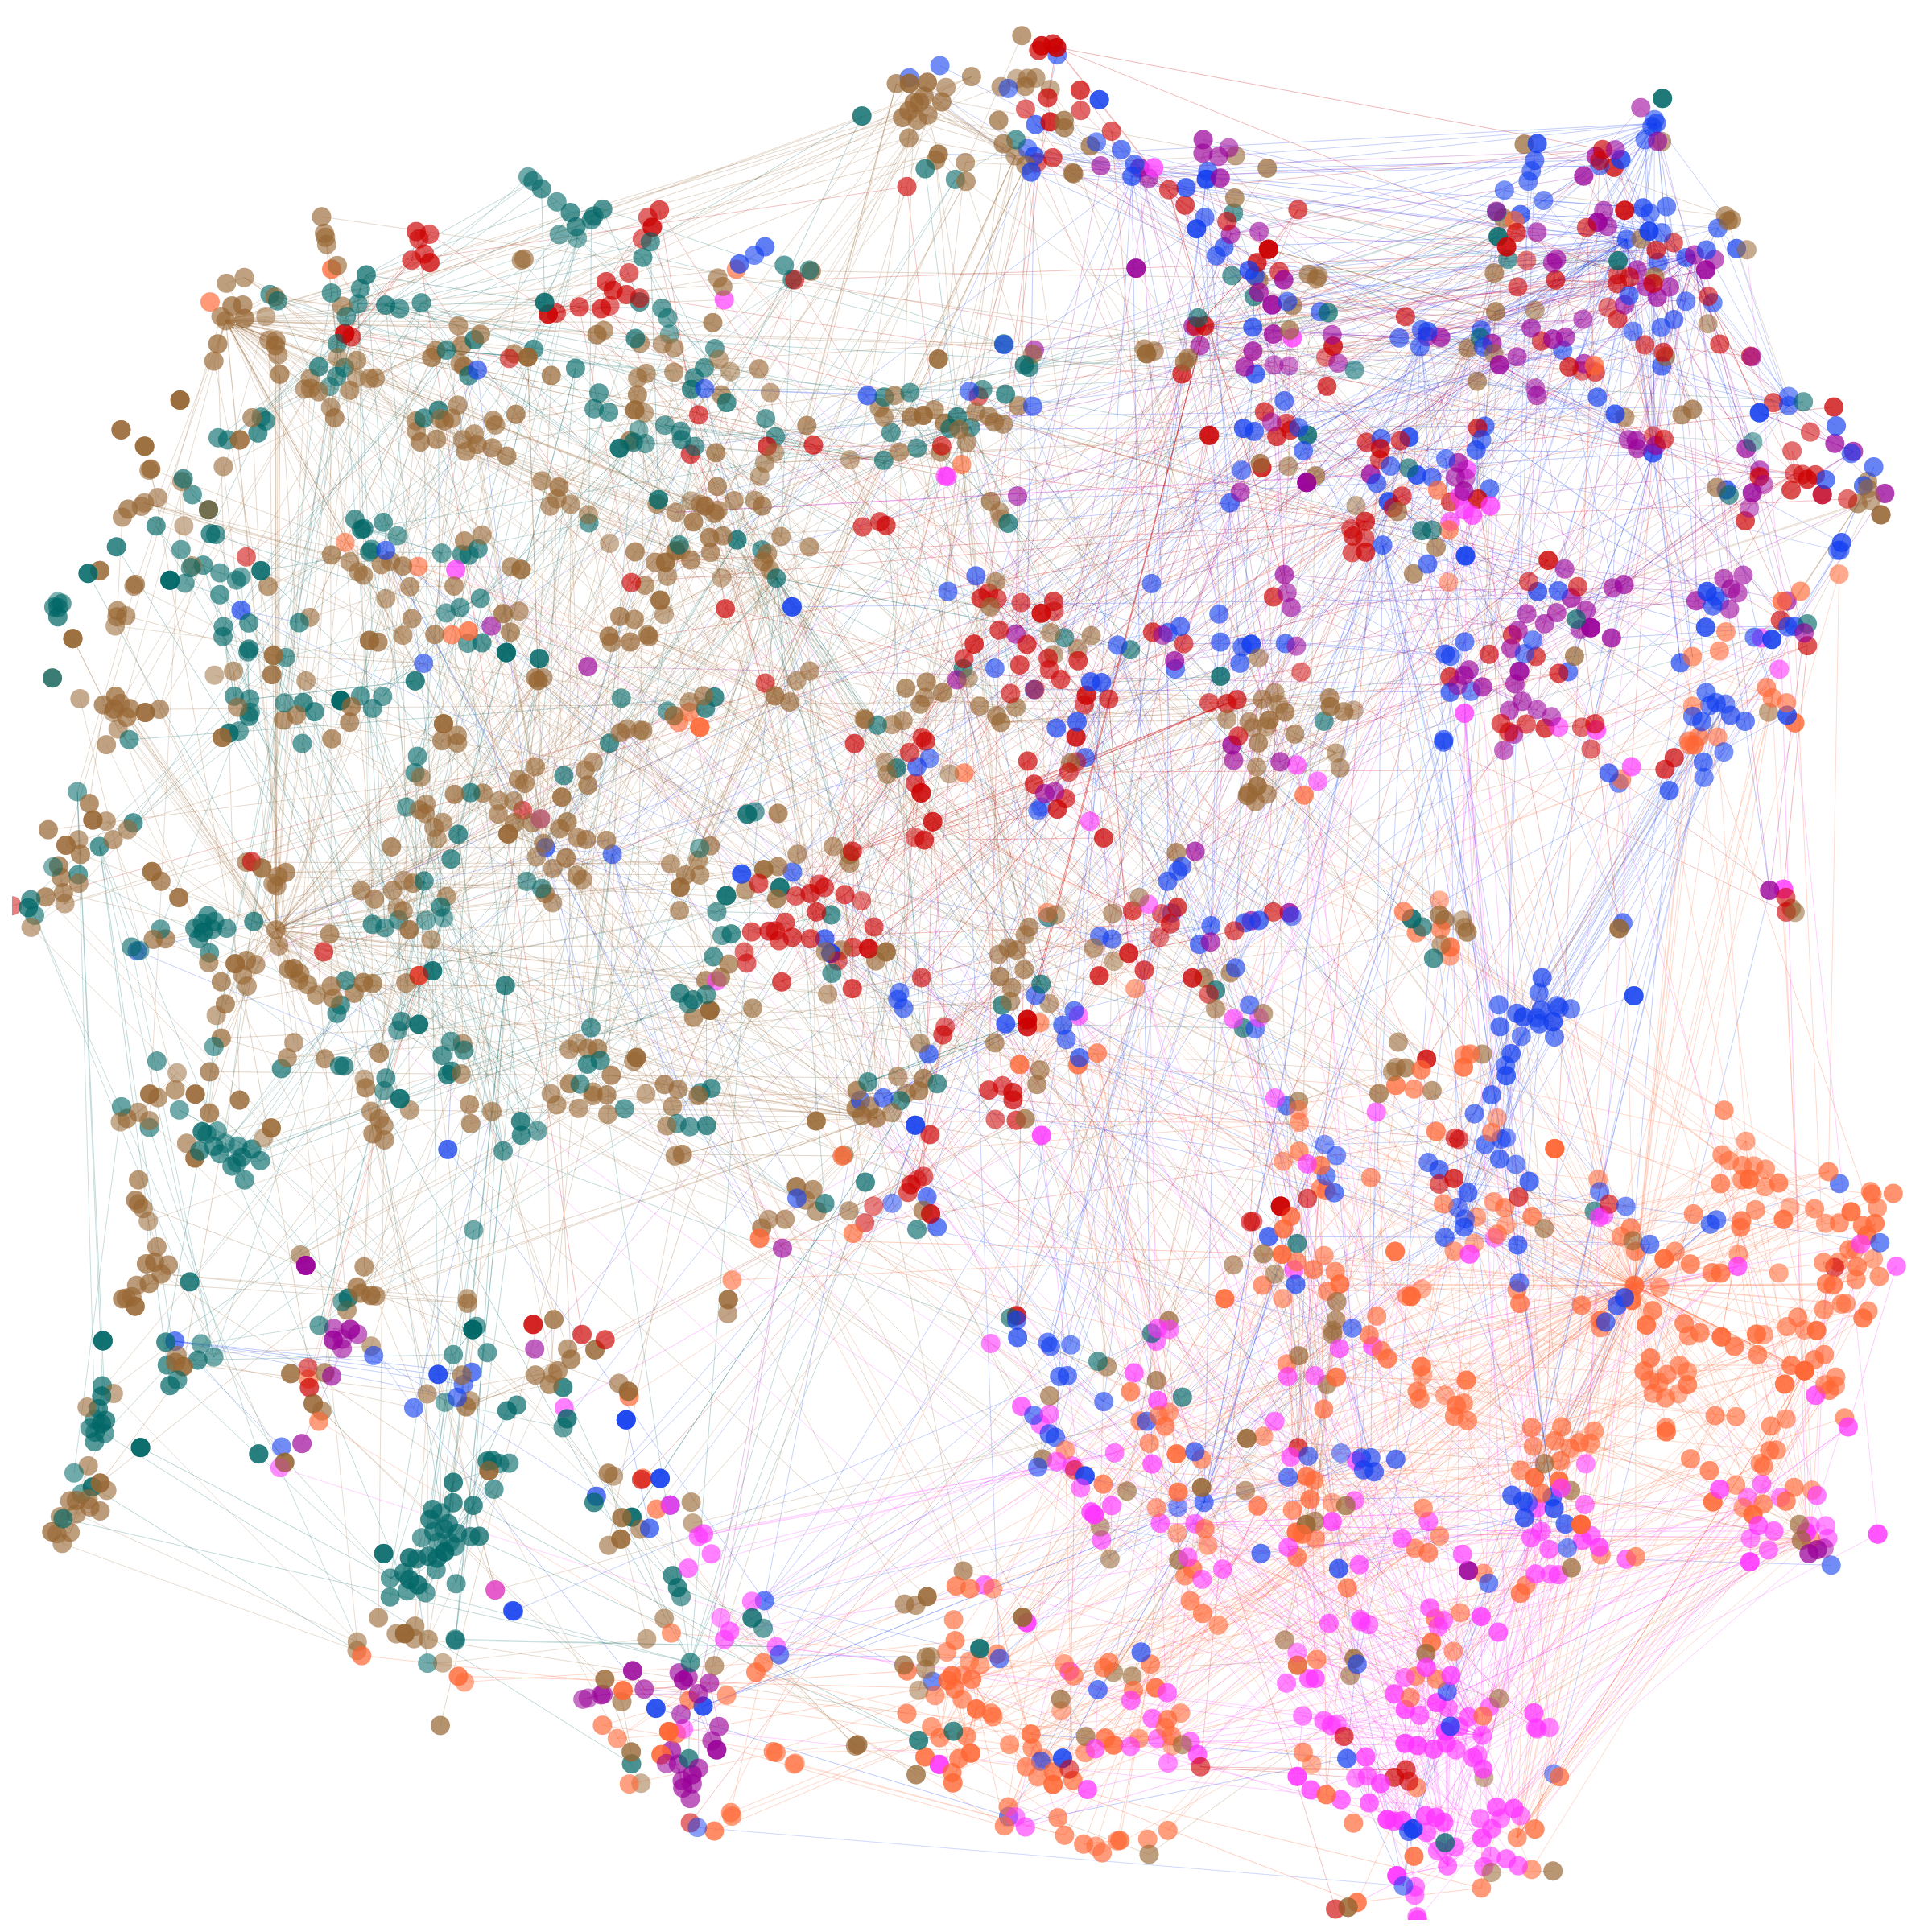
\includegraphics[width=0.20\linewidth]{figure/GCN_cora_visualization.png}
%\caption{fig1}
}%
\hspace{15pt}
\subfigure[GAT]{
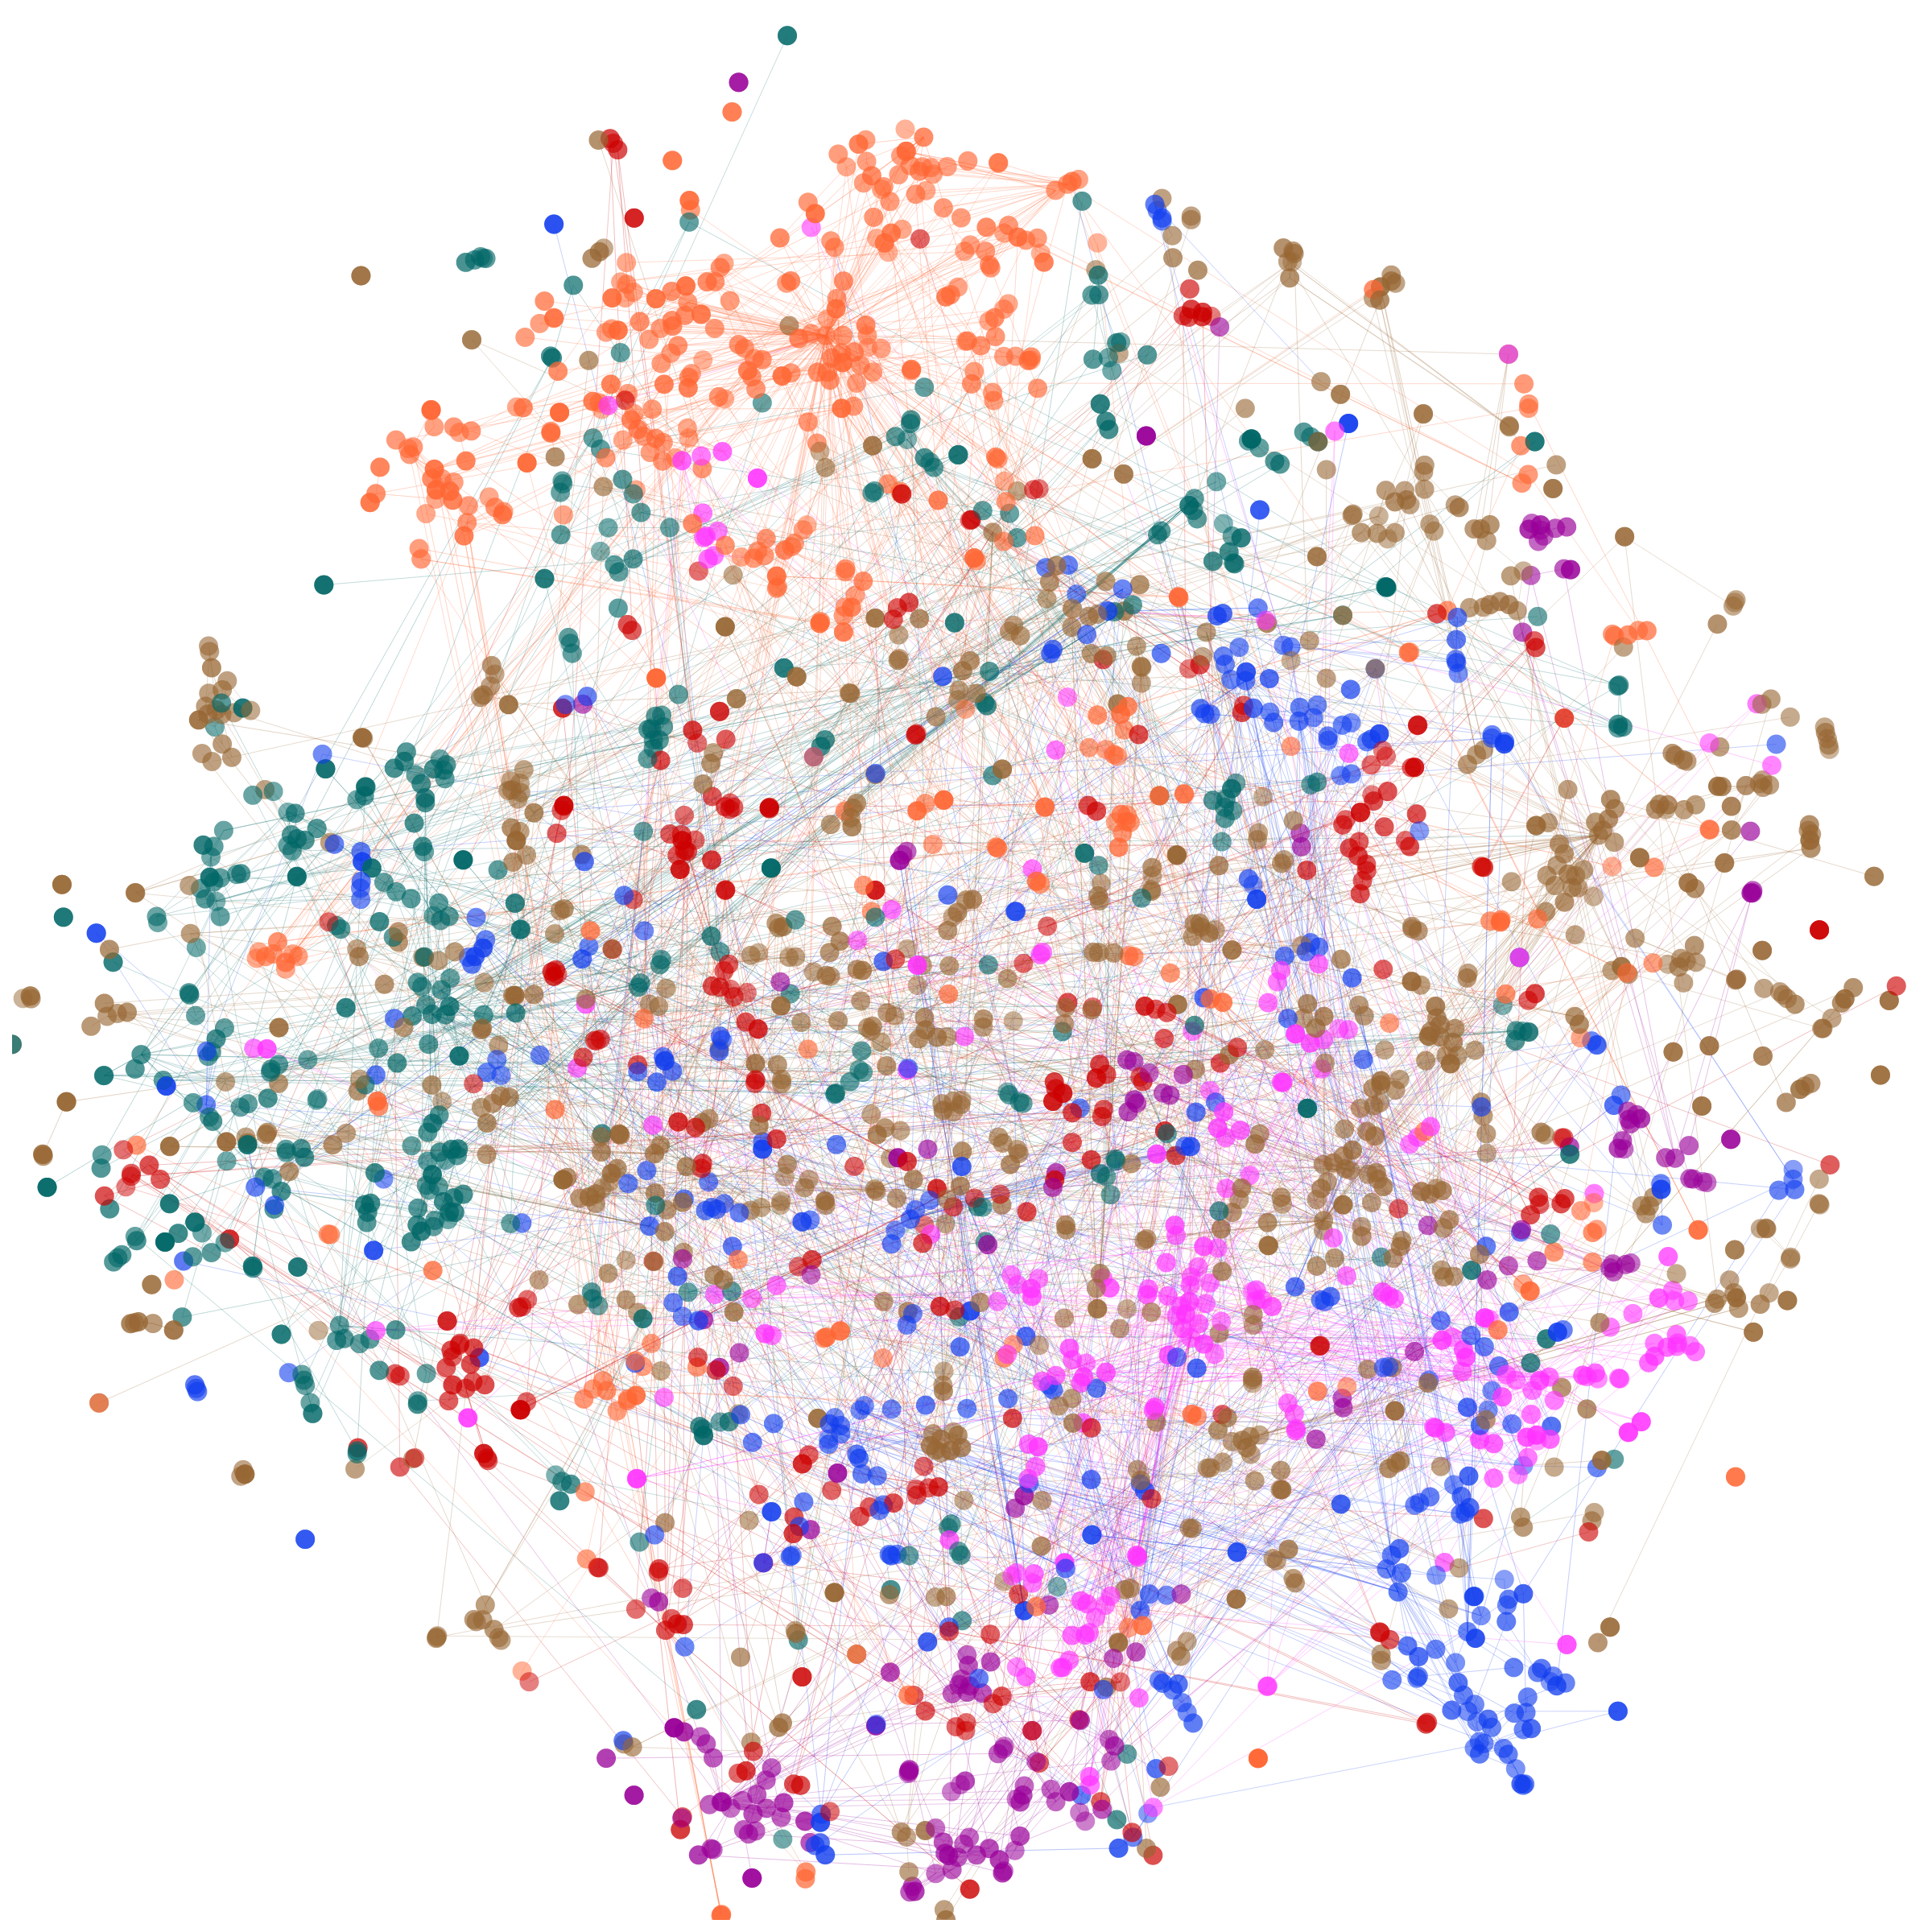
\includegraphics[width=0.20\linewidth]{figure/GAT_cora_visualization.png}
%\caption{fig2}
}%
\hspace{15pt}
\subfigure[HGCN ($K=-0.832$)]{
\includegraphics[width=0.20\linewidth]{figure/HGCN_cora_visualization.png}
}
\hspace{15pt}
\subfigure[RAHGNN ($K=-0.436$)]{
\includegraphics[width=0.20\linewidth]{figure/RHGNN_cora_visualization.png}
}
\centering
\caption{Visualization of node embeddings of different models on Cora.}
\label{visualization1}
\end{figure*}

\begin{figure*}[ht]
\centering
\subfigure[Citeseer $\delta = 4$]{
\includegraphics[width=0.15\linewidth]{figure/RHGNN_citeseer_visualization.png}
\includegraphics[width=0.15\linewidth]{figure/citeseer_att.png}
}
\subfigure[Cora $\delta = 2.5$]{
\includegraphics[width=0.15\linewidth]{figure/RHGNN_cora_visualization.png}
\includegraphics[width=0.15\linewidth]{figure/cora_att.png}
}
\subfigure[WebKB $\delta = 1$]{
\includegraphics[width=0.15\linewidth]{figure/RHGNN_webkb_visualization.png}
\includegraphics[width=0.15\linewidth]{figure/webkb_att.png}
}
\centering
\caption{Embeddings (left) and attention weights (right) visualization of RAHGNN on datasets with different $\delta$.}
\label{visualization2}
\end{figure*}

\subsection{Reinforcement Learning Analysis}
\subsubsection{RL Process Analysis.}
We plot the training process of RAHGNN to verify the effectiveness of the reinforcement learning mechanism in Figure \ref{RL_loss}, where each plot shows the trend of ROC-AUC or Accuracy for the HGNN Agent during the whole training process. The shadowed area flags min or max train metrics in a 5-fold cross validation run, and the solid line indicates the mean value. On the downstream tasks of each dataset, RAHGNN converges within a few hundred epochs.

\subsubsection{Curvature Learning analysis.}
Figure~\ref{LP-C} shows the curvature updating process of RL in different datasets and tasks. 
The blue line is the curvature of the first hyperbolic graph neural layer in HGNN, and the orange line is the curvature of the second hyperbolic graph neural layer. In most cases, when the model ends training, the curvatures also show a trend of converging to fixed values around.  We observe that the optimal curvature in the first layer is less than the one in the second layer in Pubmed and Cora with high $\delta$-hyperbolicity, while it is the opposite in WebKB and PPI with less $\delta$-hyperbolicity. 
Moreover, it is obvious that the curvatures of two HGNN layers present a close relationship with competition and cooperation: in several adjacent epochs, the curvatures of two HGNN layers often choose opposite actions simultaneously or remain unchanged at the same time; but on the scale of the entire training process, the overall trend of two layers is the same.


\begin{table}[htb]
\caption{ROC of RAHGNN with Möbius operations (RAHGNN-M) and Einstein midpoint (RAHGNN-E) for link prediction}
\begin{tabular}{lccccc}
\toprule
\textbf{Method} & \textbf{Citeseer} & \textbf{Cora} & \textbf{Pubmed} & \textbf{PPI} & \textbf{WebKB} \\ 
\midrule
RAHGNN-M         & 95.82          &  \textbf{93.22} & 93.96          & \textbf{91.60} & 93.55          \\
RAHGNN-E         & \textbf{96.94} &  91.52          & \textbf{94.87} & 91.30          & \textbf{94.32} \\ 
\bottomrule
\end{tabular}
\label{ablation}
\end{table}

\subsection{Model Analysis}
There are two main ways to compute the feature aggregation in hyperbolic neural networks: Möbius operations~\cite{HNN:GaneaBH18,HGCN_ChamiYRL19} and Einstein midpoint~\cite{HAtt}. 
% The different between Möbius operations and Einstein midpoint is: 
The Möbius operations perform the aggregation operation by using exponential mapping to project embeddings into the tangent space, and then projecting back to the hyperbolic space by logarithmic mapping. 
The Einstein midpoint is computed directly in hyperbolic space, equivalent to the weighted sum of Euclidean space. 
We further analyze the effect of two hyperbolic aggregation operations of graph in our proposed framework, namely RAHGNN+M (RAHGNN with Möbius operations) and RAHGNN+E (RAHGNN with Einstein Midpoint). 
We observe different aggregation performance of graph via these two computation operations in hyperbolic space with different curvature.
As shown in Table~\ref{ablation}, the performance of RAHGNN+E is similar to RAHGNN+M, but RAHGNN+E has a slight advantage in our experiments. 



\subsection{Visualization}
For a more intuitive comparison and to further show the effectiveness of our proposed model, we show the visualization of Cora in Figure~\ref{visualization1}. 
We visualize the embeddings of nodes in the test set by t-SNE~\cite{van2008visualizing}. The nodes are labeled with 7 different colors. 
As shown in Figure~\ref{visualization1}, HGCN and RAHGNN cluster nodes in a better separation way compared with the results of GCN and GAT. 
In contrast to HGCN, RAHGNN indicates higher intra-class similarity and the clearer distinct boundaries among different classes. 

Figure \ref{visualization2} illustrates the corresponding embeddings and attention weights in and the 2-hop neighborhood of a center node (red) for three datasets with various $\delta$. 
We visualize the attention weights for the red nodes. 
The hierarchy of the nodes are visualized by the darkness of the color. 
The intensity of edges between the neighbours denotes the attention weights of nodes. 
We observe that the center nodes are more concerned about their (grand)parents in datasets with lower $\delta$. 
In contrast to Citeseer, the aggregations with attention in Cora and WebKB pay more attention to the high hierarchy of nodes. 
Such attention is vital to good performance in datasets with different hierarchies.

\section{Related Work}\label{section 2}
% There have been many works that utilize GCNs to extract local features to preserve high-order structure patterns. 
% \cite{AbuElHaija2019MixHopHG} mixes first-order and high-order feature representations of neighbors repeatedly in each layer. 
% \cite{motif2019} selects a few motifs for each node for aggregation. 
% \cite{Jin_Song_Shi_2020} captures complex structure patterns by anonymous walks. 
% \cite{topic2020} uses topic models to pre-select anchors to discover representative structure patterns and guide the aggregation. 

Hyperbolic geometric space was introduced into complex networks earlier to represent the small world and scale-free of complex networks~\cite{Krioukov2010Hyperbolic,papadopoulos2012popularity}. 
In the real world, complex networks are generally tree-like networks and hyperbolic geometric space is used to represent two important properties of such networks: the exponential expansion of network scale and the network hierarchy~\cite{Krioukov2010Hyperbolic}. 
With high capacity and hierarchical structure-preserving ability of hyperbolic space, it is recently introduced into graph neural networks~\cite{HGNN_Qi,HGCN_ChamiYRL19,HAT}. 
To the best of our knowledge, only a few studies have considered the balance of topological structure and feature information of graph data. 

\section{Conclusion}
In this work, we proposed RAHGNN, a novel adaptive node embedding framework by reinforcement learning in hyperbolic geometric space, and we practice this framework based on the hyperboloid model. 
For graphs of different hierarchical topologies, the adaptively selected curvature can provide a good trade-off and fusion between the hierarchy and features of different graph data. 
Moreover, the curvature selection can also intuitively give a reasonable interpretation of model learning, reflecting the model preference to capture information between the structure and features of a graph. 
The proposed RAHGNN is evaluated on datasets with different hierarchical topologies for different tasks, and the experiment results show the effectiveness of our approach. 




% \begin{acks}
% To Robert, for the bagels and explaining CMYK and color spaces.
% \end{acks}

%%
%% The next two lines define the bibliography style to be used, and
%% the bibliography file.
\bibliographystyle{ACM-Reference-Format}
\bibliography{sigconf}

%%
%% If your work has an appendix, this is the place to put it.
\appendix



\end{document}
\endinput
%%
%% End of file `sample-sigconf.tex'.
